\newgeometry {margin=4cm, hmargin= 2cm}
\chapter{Espacio de la pantalla}
\section{Conversión a coordenadas de la pantalla}
Una vez se tienen las coordenadas de los puntos entre las coordenadas (-1, -1) y (1, 1) se busca encontrar la coordenada correspondiente en la pantalla.
\begin{itemize}
  \item{\(x_d\) es la coordenada en la pantalla}
  \item{\(x_s\) es la coordenada real normalizada}  
  \item{\(x_m\) es la coordenada donde comienza la superficie en la que queremos dibujar}
  \item{\(x_M\) es la coordenada donde termina la superficie en la que queremos dibujar}  
  \item{\(\Delta x = x_M - x_m\)}
\end{itemize}
\begin{equation*}
  \frac{x_s-(-1)}{1-(-1)} = \frac{x_d - x_m}{\Delta x}
\end{equation*}
Si aislamos \(x_d\) obtenemos la siguiente ecuación:
\begin{equation*}
  x_d = \frac{\Delta x \cdot x_s}{2}+\frac{\Delta x}{2}+x_m
\end{equation*}
En el caso de la coordenada \(y\) funciona igual excepto que cambiamos el sentido así que tiene una pequeña variación.
\begin{equation*}
  y_d = \frac{-(\Delta y) \cdot y_s}{2}+\frac{\Delta y}{2}+y_m
\end{equation*}
Y en forma de matriz, la operación quedaría así.

\begin{equation*}
  \begin{bmatrix}
     \frac{\Delta x}{2} && 0 && \frac{\Delta x}{2} + x_m\\
     0 && - \frac{\Delta y}{2} && \frac{\Delta y}{2} + y_m \\
     0 && 0 && 1
  \end{bmatrix}
  \cdot
  \begin{bmatrix}
    x_s\\
    y_s\\
    1
  \end{bmatrix}
  =
  \begin{bmatrix}
    x_d\\
    y_d\\
    1
  \end{bmatrix}
\end{equation*}
\restoregeometry

\section{Funcionamiento de SDL2}
Uno de los objetivos de este Treball de Recerca era utilizar una librería que permitiera compilar y ejecutar el programa en los principales Sistemas Operativos y entornos de desarrollo.

SDL2 es una librería de desarrollo multi-plataforma, que proporciona acceso de nivel bajo al audio, teclado, ratón y hardware gráfico utilizando OpenGL.

Es por eso que ha sido de vital importancia, ya que nos ha permitido simular el funcionamiento de OpenGL sin necesidad de tener que recrear partes más técnicas y complejas que no tenían relevancia en este proyecto.

En general, ha permitido crear, de forma sencilla, un entorno sobre el que aplicar la librería gráfica (tanto la de OpenGL como la nuestra propia).

\subsection{Cómo lo he usado}
SDL2 ofrece dos métodos para la gestión de gráficos, en uno se utiliza OpenGL directamente, se llama a funciones de OpenGL y se trabaja como lo haría OpenGL.

Sin embargo, también existe un método en el que OpenGL se limita a funcionar como comunicador a la tarjeta gráfica.

Este doble funcionamiento ha sido vital, pues ha permitido crear dos versiones del programa. En la primera, OpenGL se usa plenamente. En la segunda, todas las funciones de OpenGL se han mimetizado para intentar comprender cuál es su funcionamiento. Esto ha permitido crear comparaciones entre las dos versiones.


Ahora se explicarán algunas de las funciones de SDL2 que se han ido usando a lo largo del código y que hace falta definir. Para explorar estas funciones y SDL2 en general, existe un sitio oficial\footnote{https://wiki.libsdl.org} que funciona a modo de documentación.


\subsection{Funciones importantes de SDL2 - OpenGL}
Estas son las funciones relevantes para la versión del programa que utiliza plenamente OpenGL.


\subsubsection{Inicialización de SDL2}
Para iniciar un entorno de SDL2 se llama a la siguiente función:
\begin{lstlisting}[language=C]
  int SDL_Init(Uint32 flags)
\end{lstlisting}
Como parámetro, se pueden añadir flags de inicialización como por ejemplo
\textit{SDL\_INIT\_VIDEO}, para inicializar el vídeo.

\subsubsection{Creación de ventana}
Para crear una ventana se llama a esta función:
\begin{lstlisting}[language=C]
  SDL_Window* SDL_CreateWindow(const char* title,
                              int x, int y, int w, int h, 
                              Uint32 flags)
\end{lstlisting}
Donde los parámetros son el título, las coordenadas \textit{x} y \textit{y} iniciales, w y h son la anchura y la altura, respectivamente y además se puede añadir alguna opción en flag, en este caso, es necesario añadir SDL\_WINDOW\_OPENGL para indicar que esta ventana se destinará a OpenGL.

\subsubsection{Creación de contexto}
En la anterior función se creó la ventana, pero ahora hace falta crear el entorno (contexto) de renderización de OpenGL.
\begin{lstlisting}[language=C]
  SDL_GLContext SDL_GL_CreateContext(SDL_Window* window)
\end{lstlisting}
El único parámetro es la ventana previamente creada en la cuál queremos crear el contexto de renderización.

\subsubsection{Actualización de la ventana}
Puesto a que se está utilizando OpenGL será necesario llamar a
\begin{lstlisting}[language=C]
  void SDL_GL_SwapWindow(SDL_Window* window)
\end{lstlisting}
Con esta función se actualizará la ventana actual con el búfer\footnote{Espacio de memoria en el que se almacenan los datos de forma temporal} de OpenGL.

\subsubsection{Finalización de SDL2}
Una vez que se desea terminar con la ejecución del programa, hay que terminar antes el entorno de SDL2 con las siguientes funciones.
\begin{lstlisting}[language=C]
  void SDL_DestroyWindow(SDL_Window* window)
\end{lstlisting}
El único parámetro es la ventana que se desea finalizar.
\begin{lstlisting}[language=C]
  void SDL_Quit()
\end{lstlisting}

Para la demás funcionalidad, hay que referirse a OpenGL.

\subsection{Funciones importantes de SDL2 - sin OpenGL}
\subsubsection{Inicialización de SDL2}
Para iniciar un entorno de SDL2 se llama a la siguiente función:
\begin{lstlisting}[language=C]
  int SDL_Init(Uint32 flags)
\end{lstlisting}
Como parámetro, se pueden aladir flags de inicialización como por ejemplo \textit{SDL\_INIT\_VIDEO}, para inicializar el vídeo.

\subsubsection{Creación de ventana}
Para crear una ventana se llama a esta función:
\begin{lstlisting}[language=C]
  SDL_Window* SDL_CreateWindow(const char* title,
                               int x, int y, int w, int h,
                               Uint32 flags)
\end{lstlisting}
Donde los parámetros son el título, las coordenadas \textit{x} y \textit{y} iniciales, w y h son la anchura y la altura, respectivamente y además se puede añadir alguna opción en flag.

\subsubsection{Creación de renderizador}
Puesto a que no estamos utilizando OpenGL de forma directa, es necesario crear un Renderer que gestione lo que SDL tiene que dibujar.
\begin{lstlisting}
  SDL_Renderer* SDL_CreateRenderer(SDL_Window* window,
                int index, Uint32 flags)
\end{lstlisting}
El primer parámetro es la ventana en la que se desea dibujar, la segunda es el índice del dispositivo de renderización (medio que se quiere utilizar para los gráficos) y finalmente una flag que indique el tipo de renderización a usar.


\subsubsection{Cambio de color}
En lugar lugar de escoger el color cada vez que se dibuja algo, SDL2 guarda el último color seleccionado y es el que utiliza hasta que se llama a la siguiente función.
\begin{lstlisting}[language=C]
  void SDL_SetRenderDrawColor(SDL_Renderer* renderer,
       int8 r, Uint8 g, Uint8 b, Uint a)
\end{lstlisting}
El primer parámetro es el contexto de renderización que se está utilizando, y los siguientes son los valores RGBA, que definen el color y oscilan del 0 al 255 cada uno.

\subsubsection{Dibujo de puntos}
Para dibujar un punto, simplemente hay que usar la siguiente función.
\begin{lstlisting}[language=C]
  int SDL_RenderDrawPoint(SDL_Renderer* renderer,
                         int x, int y)
  
\end{lstlisting}
El primer parámetro es el contexto usado actualmente. Los valores \textit{x} y \textit{y} corresponden a la coordenada de la pantalla en la que se desea dibujar un punto.

\subsubsection{Dibujo de líneas}
Para dibujar una línea, funciona de forma similar a un punto, pero con una coordenada adicional (la final).
\begin{lstlisting}[language=C]
  int SDL_RenderDrawLine(SDL_Renderer* renderer,
                        int x1, int y1,
                        int x2, int y2)
\end{lstlisting}
El primer parámetro es el contexto de renderización que se está utilizando, \textit{x1} y \textit{y1} corresponden a la coordenada origen de la línea y \textit{x2} y \textit{y2} corresponden a la coordenada final de la línea.


En caso de de no estar utilizando OpenGL directamente, se puede llamar a
\begin{lstlisting}[language=C]
  void SDL_RenderPresent(SDL_Renderer* renderer)
\end{lstlisting}
El único parámetro es el renderer utilizado actualmente.

\subsubsection{Actualización de la ventana}
Una vez se hayan aplicado todas las operaciones que se deseen, se ha de llamar a la siguiente función para mostrarlo.
\begin{lstlisting}[language=C]
  void SDL_RenderPresent(SDL_Renderer* renderer)
\end{lstlisting}
El único parámetro es el renderizador que se quiere actualizar.
\newpage

\subsubsection{Finalización de SDL2}
La forma de finalizar SDL2 cuando no se ha usado directamente OpenGL es un poco más compleja.
Primero hace falta destruir el renderer que se ha usado.
\begin{lstlisting}[language=C]
  void SDL_DestroyRenderer(SDL_Renderer* renderer)
\end{lstlisting}
Posteriormente, se destruye la ventana.
\begin{lstlisting}[language=C]
  void SDL_DestroyWindow(SDL_Window* window)
\end{lstlsiting}

Finalmente, se cierra el entorno de SDL.
\begin{lstlisting}[language=C]
  void SDL_Quit()
\end{lstlisting}

\section{Estructura del código}

\begin{figure}[h]
 \centering
 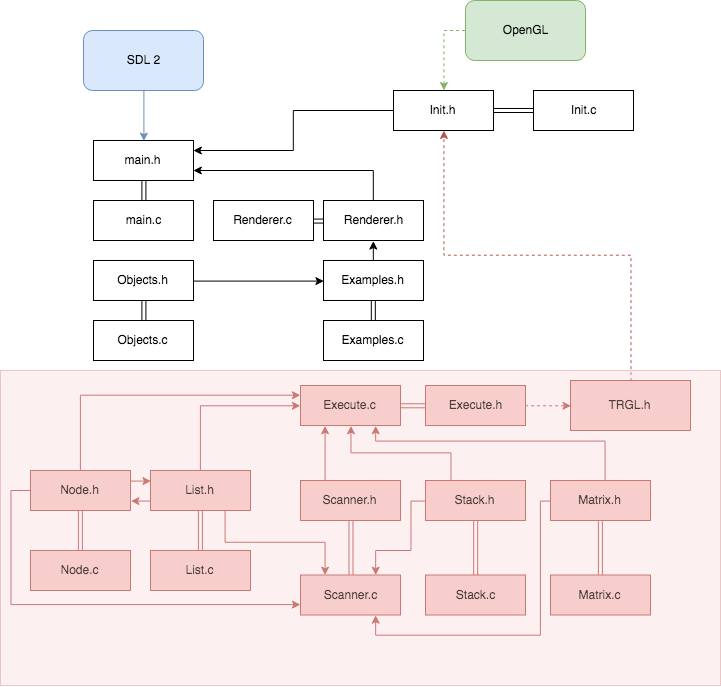
\includegraphics[width=\textwidth]{diagrama}
\end{figure}

\begin{itemize}
  \item{main: es donde se inicia la lógica de SDL (la gestión de
      ventanas y se llaman a las demás funciones del programa}
  \item{Init: contiene muchos aspectos de la inicialización del motor
      gráfico y es la parte que se dedica a decidir entre OpenGL y
      TRGL}
  \item{Renderer: contiene el bucle general de renderización, adema´s
      de algunas funciones que han sido deprecadas pero que se querían
      implementar}
  \item{Objects: algunas formas geométricas}
  \item{Examples: funciones con muestras de lo que se puede
      renderizar}
  \item{TRGL: sustituye parte de la funcionalidad de OpenGL}
  \item{Node: estructuras de memoria donde se guarda información concreta}
  \item{List: estructuras de memoria en las que se guardan nodos}
  \item{Matrix: recursos matemáticos para la gestión de matrices}
  \item{Scanner: lector de las estructuras de memoria}
  \item{Execute: intérprete de la información leída}
\end{itemize}